\documentclass[12pt,aspectratio=169,notheorems]{beamer}
\graphicspath{
	{img}
}

\usetheme[progressbar=frametitle, numbering=fraction]{metropolis}
\usepackage{appendixnumberbeamer}
\usepackage[font=small,labelfont=bf]{caption}
\usepackage{hyperref}
\usepackage{multirow}
\setbeamercolor{background canvas}{bg=white}

\usepackage{booktabs}
\usepackage[scale=2]{ccicons}

% Change Color of the theme
\usepackage{xcolor}
\definecolor{DarkGrey}{HTML}{353535}
\definecolor{ECNURed}{RGB}{164,31,53}
\definecolor{ECNUBrown}{RGB}{134,117,77}
\setbeamercolor{normal text}{ fg= DarkGrey  }
\setbeamercolor{alerted text}{ fg= ECNURed  }
\setbeamercolor{example text}{ fg= ECNUBrown  }



\title{\LARGE AI Project Report}
\subtitle{Network Intrusion Detection System}
\author{\\ Andrea Mugnai \\ Jacopo Tucci}
\date{2024/2025}
\titlegraphic{\hfill
\includegraphics[height=2cm]{logo.png}}

\begin{document}

\maketitle

\begin{frame}{Goals}
    Our goal is to create a Network Intrusion Detection System (NIDS) capable of classifying raw network packets into the following categories:
    \begin{itemize}
        \item Normal
        \item Denial of Service (DoS)
        \item User to Root (U2R)
        \item Remote to Local (R2L)
        \item Probe
    \end{itemize}
    The classification models used for this task are based on \textbf{supervised learning}.
\end{frame}

\begin{frame}{Dataset}
    We used a non cleaned dataset: \href{https://research.unsw.edu.au/projects/unsw-nb15-dataset}{UNSW-NB15}. 
    The raw packet was created by the \texttt{IXIA PerfectStorm tool}. This dataset is a labeled datset and in particular has nine types of attacks 
    that we mapped in the categories we mentioned before as follows:
    \begin{itemize}
        \item DoS: DoS, Worms.
        \item U2R: Backdoor, Shellcode.
        \item R2L: Exploits, Analysis.
        \item Probe: Reconnaissance, Fuzzers, Generic.
        \item Normal: Benign packets.
    \end{itemize}
        \small We used the \texttt{label} column to map the attacks to categories. In particular all the \texttt{attack\_cat} values were empty for the \texttt{Normal} class. \\
\end{frame}

\begin{frame}{Category Distribution}
        \centering
        \footnotesize The dataset is highly unbalanced, with the majority of the samples \\
        belonging to the \textbf{Normal} class.
    \begin{center}
        \hspace*{-1.5cm}
        \begin{minipage}[t][6cm][t]{0.5\textwidth}
            \centering
            \vspace{-0.08cm}
            \resizebox{1.2\textwidth}{!}{
                \begin{table}[]
                \begin{tabular}{|l|l|l|l|l|l|l|l|l|l|}
                \hline
                \textbf{Normal}               & \textbf{Generic}           & \textbf{Exploits}          & \textbf{Fuzzers}           & \textbf{Reconnaissance}    & \textbf{DoS}               & \textbf{Backdoor}        & \textbf{Analysis}        & \textbf{Shellcode}       & \textbf{Worms}
                \\ \hline
                \multicolumn{1}{|c|}{281462} & \multicolumn{1}{c|}{6894} & \multicolumn{1}{c|}{6851} & \multicolumn{1}{c|}{4970} & \multicolumn{1}{c|}{3420} & \multicolumn{1}{c|}{1465} & \multicolumn{1}{c|}{623} & \multicolumn{1}{c|}{621} & \multicolumn{1}{c|}{371} & \multicolumn{1}{c|}{42}
                \\ \hline
                \end{tabular}
                \end{table}
                \caption{Counts for each attack category.}
                \label{tab:inverted_attack_categories}
            }
            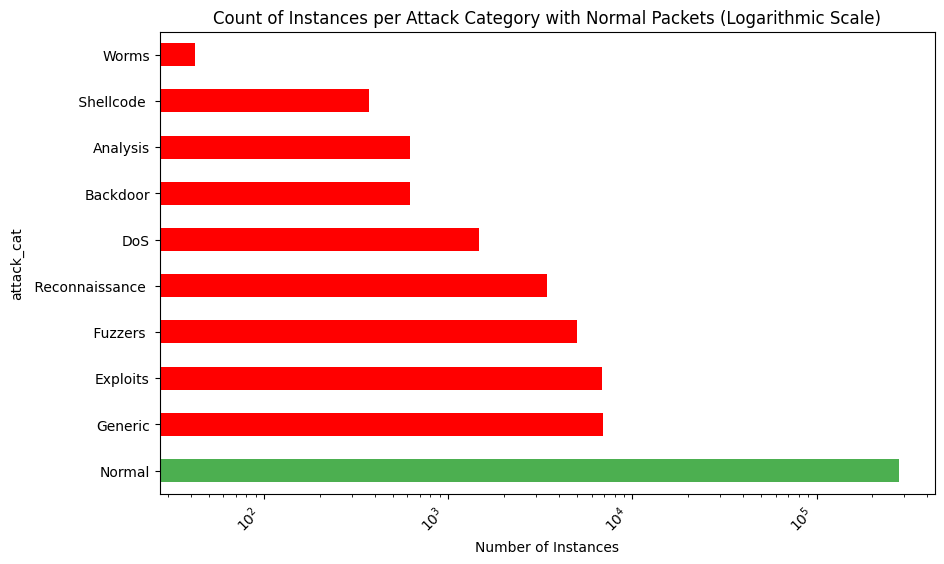
\includegraphics[width=\textwidth, height=5cm, keepaspectratio]{attack_cat_before.png} \\
            \textit{Original Dataset \emph{attack category} distribution}
        \end{minipage} 
        \hspace{0.8cm}
        \begin{minipage}[t][6cm][t]{0.5\textwidth}
            \centering
            \vspace{-0.08cm}
            \resizebox{0.5\textwidth}{!}{
                \begin{table}[]
                \begin{tabular}{|l|l|l|l|l|}
                \hline
                \textbf{Normal}               & \textbf{Probe}           & \textbf{R2L}          & \textbf{DoS}           & \textbf{U2R}
                \\ \hline
                \multicolumn{1}{|c|}{281462} & \multicolumn{1}{c|}{15284} & \multicolumn{1}{c|}{7472} & \multicolumn{1}{c|}{1507} & \multicolumn{1}{c|}{994}
                \\ \hline
                \end{tabular}
                \end{table}
                \caption{Counts for each attack category.}
                \label{tab:inverted_attack_categories}
            }
            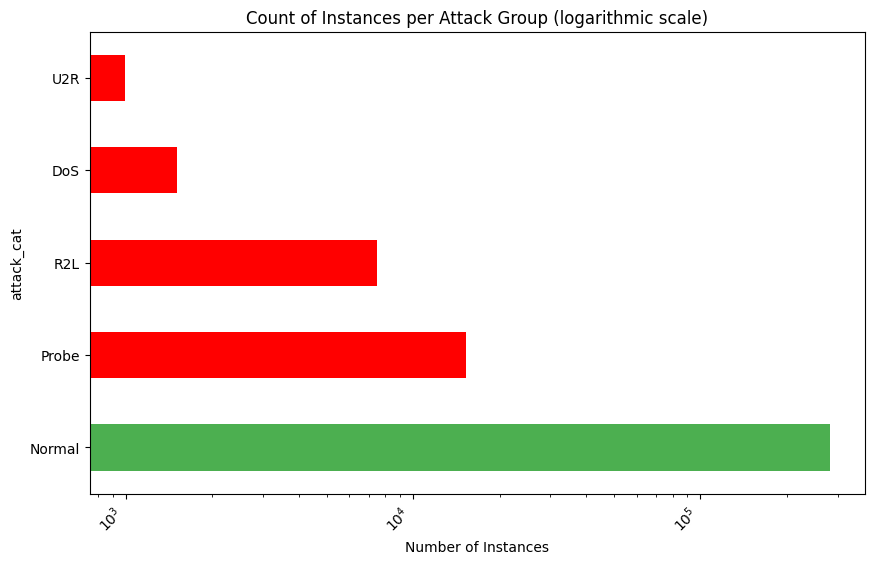
\includegraphics[width=\textwidth, height=4.2cm, keepaspectratio]{attack_cat_after.png} \\
            \textit{Our Dataset \emph{attack category} distribution}
        \end{minipage}
        \hspace*{-1cm}
    \end{center}
\end{frame}

\begin{frame}{Identify Missing and Erroneus Values }
        \scriptsize 
        We identified 49 features in the dataset, 42 of which are numerical and 7 are categorical.
        The Dataset contained missing values: 
        \begin{table}[]
            \centering
            \resizebox{0.5\textwidth}{!}{%
                \begin{tabular}{|l|l|l|l|l|}
                \hline
                               & ct\_flw\_http\_mthd & is\_ftp\_login & service & ct\_ftp\_cmd\\ \hline
                Missing Values & 273700              & 300350         & 167857 & 300350 \\ \hline
                \end{tabular}%
            }
        \end{table}        
        The \emph{attributes }\texttt{ct\_flw\_http\_mthd} indicates how many \emph{HTTP} method are present is correlated with 
        the value \textt{http} in \texttt{service} but we found a discrepancy:
        \begin{table}[]
            \centering
            \resizebox{0.4\textwidth}{!}{%
                \begin{tabular}{|l|l|l|l|}
                \hline
                               & ct\_flw\_http\_mthd & service 'http' \\ \hline
                Count Values & 33019             & 32777  \\ \hline
                \end{tabular}%
            }
        \end{table}
        This means that the differences '242' that are signed as missing in \texttt{service} can be set to \texttt{http}.  \\
        \vspace{2ex}
        Analysing the attributes \texttt{is\_ftp\_login}, \texttt{ct\_ftp\_cmd} we notice that they are equals in number, in values and in raws.  
        Probably one of them is wrong, even if not anyway the attributes together are redundant.
        \vspace{2ex}\\
        So we filled with \emph{"missing"} the \texttt{service} attribute and we filled with \emph{0} \texttt{ct\_ftp\_cmd} and \texttt{ct\_flw\_http\_mthd}.
\end{frame}

\begin{frame}{Feature Selection}
    First we removed the following columns:
    \begin{itemize}
        \item Source and Destination IP addresses (\texttt{srcip, dstip}).
        \item Source and Destination Port (\texttt{sport, dsport}).
        \item \texttt{is\_ftp\_login}.
    \end{itemize}
    We dropped the duplicates. Then we adopted two different feature selection methods:
    \begin{itemize}
        \item \textbf{Logistic Regression}: We eliminated the features with a correlation higher than 0.8 among them.
        \item \textbf{Random Forest}: We used a \textbf{Decision Tree} model to estimate the coefficient of the most important feature for constructing the tree. We dropped the others.
    \end{itemize}
\end{frame}

\begin{frame}{Feature Selection}
    \vspace{2ex}
    \hspace*{-0.8cm}
    \begin{minipage}[t]{0.45\textwidth} 
        \centering
        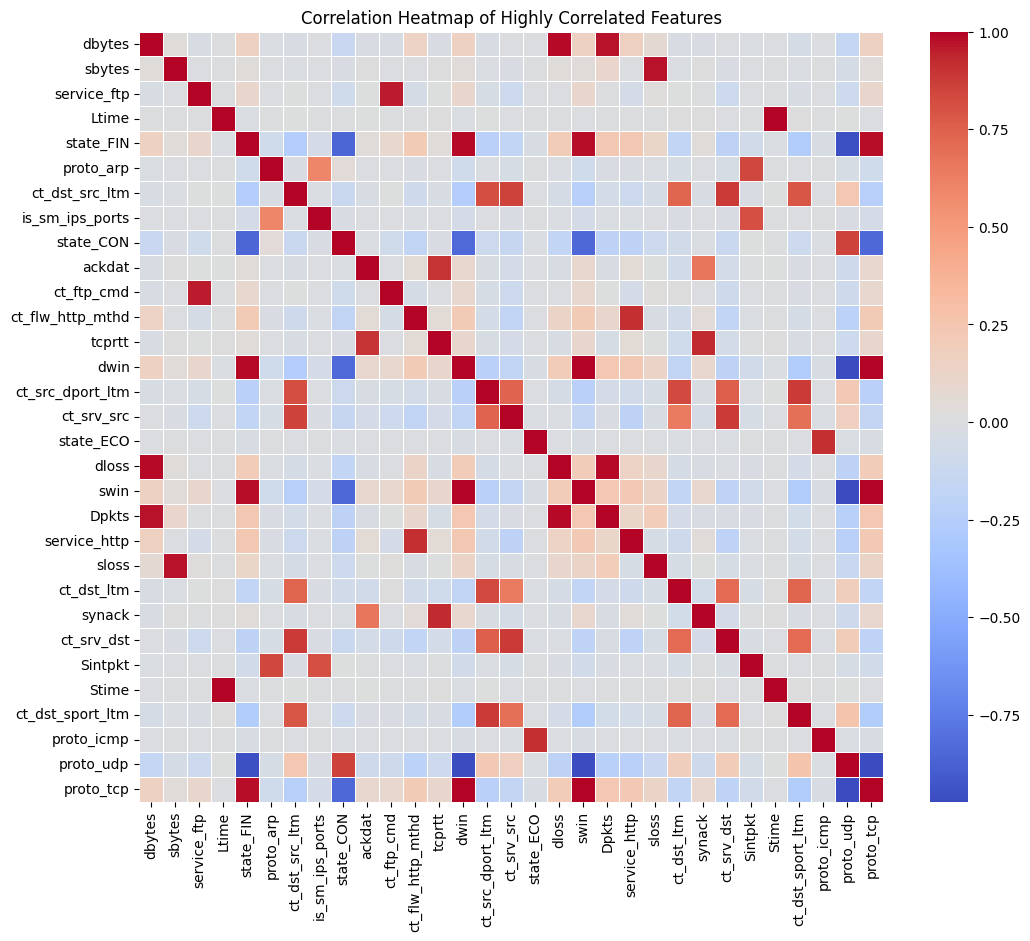
\includegraphics[width=\textwidth]{Correlation_matrix.png}
        \hspace{-1cm}
        \hspace{20cm}\subcaption{\textbf{Figure 1:} Correlation matrix}
    \end{minipage}
    \hspace{0.5cm}
    \begin{minipage}[t]{0.45\textwidth}
        \centering
        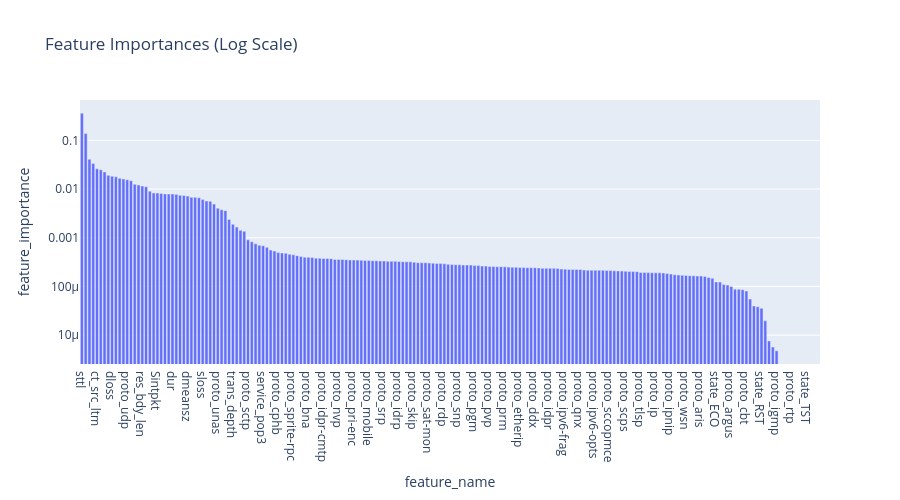
\includegraphics[width=1.4\textwidth]{DT_features_importance.png}
        \hspace{20cm}\subcaption{\textbf{Figure 2:} Feature importance for Decision Tree}
    \end{minipage}
\end{frame}

\begin{frame}{Data Preparation}
    \small As shown before the dataset is highly unbalanced with respect to the \texttt{Normal} class. 
    \vspace{-0.1cm}
        \begin{table}[t]
            \resizebox {0.35\textwidth}{!}{
            \begin{tabular}{|l|l|l|l|l|}
                \hline
                \textbf{Normal}               & \textbf{Probe}           & \textbf{R2L}          & \textbf{DoS}           & \textbf{U2R}
                \\ \hline
                \multicolumn{1}{|c|}{281462} & \multicolumn{1}{c|}{15284} & \multicolumn{1}{c|}{7472} & \multicolumn{1}{c|}{1507} & \multicolumn{1}{c|}{994}
                \\ \hline
            \end{tabular}
            }
        \end{table}
        \vspace{-0.1cm}
        \small To minimize excessive transformations of the dataset, we first applied \emph{undersampling} to the majority class, followed by \emph{oversampling} of the others. Additionally, \emph{Stratified Cross Validation} was performed as follows:
    \begin{itemize}
        \item Data trasformation of nominal data with \emph{OneHotEncoding} (using \texttt{get\_dummies}).
        \item Performs Stratified Cross Validation with \emph{StratifiedKFold} with \emph{k = 10}.
        \item Split the dataset in training and test set to rebalancing only the first one, so
        \item Apply the \texttt{RandomUnderSampler} to reduce the \emph{Normal} class to 100000 samples.
        \item Only then apply \texttt{SMOTE} to balance the training set.
    \end{itemize}
\end{frame}

\begin{frame}{Data Processing}
    \centering
    \small Two types of models were utilized for the data processing task:
    \vspace{0.4cm}

    \begin{columns}[T]
        \column{0.48\textwidth}
        \textbf{Logistic Regression}
        \begin{itemize}
        \setlength\itemsep{-0.3em}
            \item Initially implemented for the \emph{multi-class} classification problem.
            \item Performance was suboptimal, especially for \texttt{DoS} and \texttt{U2R} attacks, due to limitations in recognizing minority classes.
            \item We attempted to use the model for binary classification.
        \end{itemize}

        \column{0.48\textwidth}
        \textbf{Random Forest}
        \begin{itemize}
        \setlength\itemsep{-0.3em}
            \item Implemented only for multi-class classification problem.
            \item The result is quite good.
            \item We employed LIME (Local Interpretable Model-agnostic Explanations) to interpret model decisions.
        \end{itemize}
    \end{columns}
\end{frame}

\begin{frame}{Logistic Regression}
        - Set the maximum number of iterations to 1000. \\
        - Unbalanced dataset. \\
        - Cross-validation with a balanced training dataset. \\
        - Experimented with frequency encoding resulting in a faster model.
        \vspace{0.2cm}
    \begin{table}[]
        \begin{tabular}{l|l|ll|}
        \cline{2-4}
            & \multicolumn{1}{c|}{\multirow{2}{*}{Unbalanace}} & \multicolumn{2}{c|}{Balance}                             \\ \cline{3-4}
            & \multicolumn{1}{c|}{}                            & \multicolumn{1}{l|}{OneHotEncoding} & Frequency Encoding \\ \hline
            \multicolumn{1}{|l|}{\textbf{Precision}} & 0.49                                             & \multicolumn{1}{l|}{0.49}           & 0.49               \\ \hline
            \multicolumn{1}{|l|}{\textbf{Recall}}    & 0.49                                             & \multicolumn{1}{l|}{0.61}           & 0.65               \\ \hline
            \multicolumn{1}{|l|}{\textbf{F1-score}}  & 0.48                                             & \multicolumn{1}{l|}{0.51}           & 0.51               \\ \hline
        \end{tabular}
        \\
        \vspace{0.4cm}
        These approaches did yield poor improvement in performance.
    \end{table}
\end{frame}

\begin{frame}{Logistic Regression}
    \vspace{0.2cm}
    \begin{columns}[T]
        \column{0.48\textwidth}
        \small{A confusion matrix example for a cross-validation fold.}
        \\
        \vspace{0.3cm}
        \begin{minipage}[t]{1\textwidth}
            \centering
            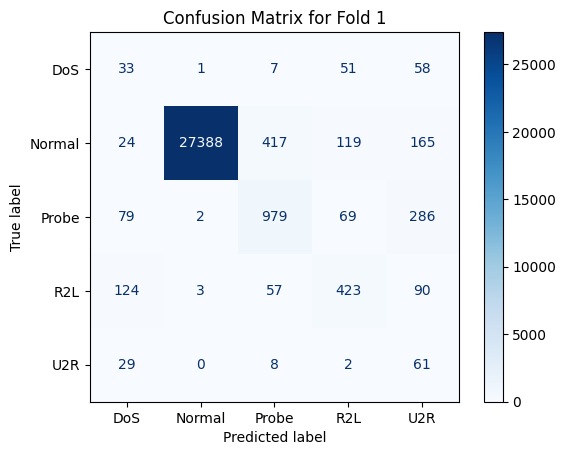
\includegraphics[width=\textwidth]{confusion_matrix_LR.png}
            \hspace{-1cm}
            \hspace{20cm}\subcaption{\small{Fold one for OHE with balanced dataset.}}
        \end{minipage}

        \column{0.48\textwidth}
        \centering
        \textbf{Binomial Logistic Regression}
        \vspace{0.2cm}
        \begin{itemize}
        \setlength\itemsep{0.5em}
            \item '1' represents an attack and '0' represents normal traffic.
            \item The results have improved significantly, as we expected.
        \end{itemize}
        \vspace{0.2cm}
        \begin{table}[]
            \begin{tabular}{|l|l|l|}
            \hline
            \multicolumn{1}{|c|}{\textbf{Precision}} & \multicolumn{1}{c|}{\textbf{Recall}} & \multicolumn{1}{c|}{\textbf{F1-score}} \\ \hline
            0.885                                    & 0.985                                & 0.928                                             \\ \hline
            \end{tabular}
        \end{table}
    \end{columns}
\end{frame}

\begin{frame}{Random Forest}
    \vspace{0.3cm}
        By using this model, we have observed improvements in performance.\\
        \vspace{0.2cm}
        \textbf{Main Parameters:} \\
        \vspace{0.1cm}
        -- Number of Trees (n\_estimators): 100 \\
        -- Splitting Criterion (default): Gini Index \\
        \vspace{0.5cm}
            \begin{columns}[T]
            \column{0.44\textwidth}
            \textbf{Macro Performance:}
            \vspace{0.2cm}
            \begin{table}[]
            \resizebox{0.8\columnwidth}{!}{
                \begin{tabular}{lll}
                \hline
                \multicolumn{1}{|c|}{\textbf{Precision}} & \multicolumn{1}{c|}{\textbf{Recall}} & \multicolumn{1}{c|}{\textbf{F1-score}} \\ \hline
                \multicolumn{1}{|l|}{0.565}              & \multicolumn{1}{l|}{0.628}           & \multicolumn{1}{l|}{0.590}             \\ \hline
                                         &                                      &
                \end{tabular}
            }
            \end{table}
            \column{0.56\textwidth}
            \textbf{First Fold Performance:}
            \vspace{0.2cm}
            \begin{table}[]
            \resizebox{0.8\columnwidth}{!}{
                \begin{tabular}{l|l|l|l|}
                \cline{2-4}
                & \multicolumn{1}{c|}{\textbf{Precision}} & \multicolumn{1}{c|}{\textbf{Recall}} & \multicolumn{1}{c|}{\textbf{F1-score}} \\ \hline
                \multicolumn{1}{|l|}{DoS}    & 0.208                                   & 0.167                                & 0.185                                  \\ \hline
                \multicolumn{1}{|l|}{Normal} & 0.998                                   & 0.984                                & 0.991                                  \\ \hline
                \multicolumn{1}{|l|}{Probe}  & 0.724                                   & 0.887                                & 0.797                                  \\ \hline
                \multicolumn{1}{|l|}{R2L}    & 0.727                                   & 0.809                                & 0.766                                  \\ \hline
                \multicolumn{1}{|l|}{U2R}    & 0.218                                   & 0.340                                & 0.266                                  \\ \hline
                \end{tabular}
            }
            \end{table}
    \end{columns}
\end{frame}

\begin{frame}{Random Forest}
    \vspace{2ex}
    \hspace*{-0.8cm}
    \begin{minipage}[t]{0.40\textwidth}
        \centering
        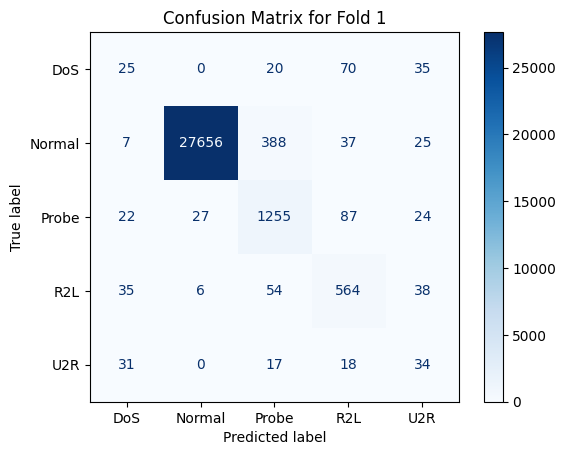
\includegraphics[width=\textwidth]{confusion_matrx_RF.png}
        \hspace{-1cm}
        \hspace{20cm}\subcaption{\textbf{First Fold Confusion Matrix}}
    \end{minipage}
    \hspace{0.5cm}
    \begin{minipage}[t]{0.45\textwidth}
        \centering
        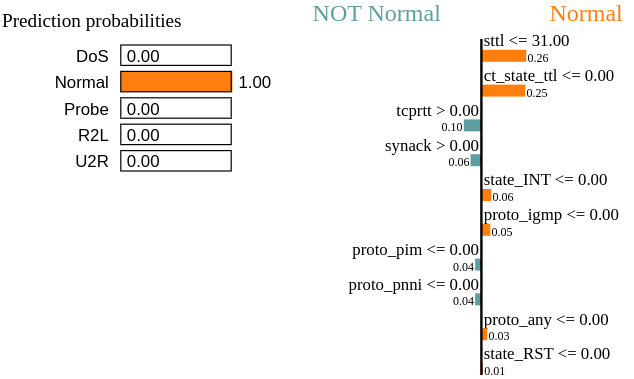
\includegraphics[width=1.4\textwidth]{lime_result.png}
        \hspace{20cm}\subcaption{\textbf{Lime Result}}
    \end{minipage}
\end{frame}

\begin{frame}{Database - ER diagram details}
    The \emph{N-to-N} relationship between \textbf{Player} and \textbf{Gacha} will be implemented with the table \textbf{Player\_Gacha}. The \textbf{Player\_Auction} table expresses the \emph{N-to-N} relationship between \textbf{Player} and \textbf{Auction}. When a player wins an auction and pays the gacha, a transaction record will be created. \\[1ex]
    Each auction is created by one player (i.e. \emph{create} relationship) and it will contain a reference to a transaction record when the winning player pays the bid. For \textbf{Transaction} records, we store the creation datetime. \\[1ex]
    The gacha's rarities are stored inside \textbf{Rarity} table and each gacha maintains a reference to a specific rarity.
\end{frame}

\begin{frame}{References}
    \begin{itemize}
        \small
        \item \href{https://unsw-my.sharepoint.com/personal/z5025758_ad_unsw_edu_au/_layouts/15/onedrive.aspx?id=\%2Fpersonal\%2Fz5025758\%5Fad\%5Funsw\%5Fedu\%5Fau\%2FDocuments\%2FUNSW\%2DNB15\%20dataset&ga=1}{Specification of \texttt{UNSW-NB15} dataset}.
        \item \href{https://ieeexplore.ieee.org/abstract/document/8470090}{"An Ensemble Intrusion Detection Technique based on proposed Statistical Flow Features for Protecting Network Traffic of Internet of Things".}
        \item \href{https://ieeexplore.ieee.org/abstract/document/7348942}{"UNSW-NB15: a comprehensive data set for network intrusion detection systems".}
    \end{itemize}   
\end{frame}

\end{document}
